% THIS DOCUMENT IS FOLLOWS THE VOLERE TEMPLATE BY Suzanne Robertson and James Robertson
% ONLY THE SECTION HEADINGS ARE PROVIDED
%
% Initial draft from https://github.com/Dieblich/volere
%
% Risks are removed because they are covered by the Hazard Analysis
\documentclass[12pt]{article}

\usepackage{booktabs}
\usepackage{xltabular}
\usepackage{hyperref}
\usepackage{graphicx}
\usepackage{multirow}
\hypersetup{
    bookmarks=true,         % show bookmarks bar?
      colorlinks=true,      % false: boxed links; true: colored links
    linkcolor=red,          % color of internal links (change box color with linkbordercolor)
    citecolor=green,        % color of links to bibliography
    filecolor=magenta,      % color of file links
    urlcolor=cyan           % color of external links
}

\newcommand{\lips}{\textit{Insert your content here.}}

%% Comments

\usepackage{color}

\newif\ifcomments\commentstrue %displays comments
%\newif\ifcomments\commentsfalse %so that comments do not display

\ifcomments
\newcommand{\authornote}[3]{\textcolor{#1}{[#3 ---#2]}}
\newcommand{\todo}[1]{\textcolor{red}{[TODO: #1]}}
\else
\newcommand{\authornote}[3]{}
\newcommand{\todo}[1]{}
\fi

\newcommand{\wss}[1]{\authornote{blue}{SS}{#1}} 
\newcommand{\plt}[1]{\authornote{magenta}{TPLT}{#1}} %For explanation of the template
\newcommand{\an}[1]{\authornote{cyan}{Author}{#1}}

%% Common Parts

\newcommand{\progname}{ProgName} % PUT YOUR PROGRAM NAME HERE
\newcommand{\authname}{Team \#, Team Name
\\ Student 1 name
\\ Student 2 name
\\ Student 3 name
\\ Student 4 name} % AUTHOR NAMES                  

\usepackage{hyperref}
    \hypersetup{colorlinks=true, linkcolor=blue, citecolor=blue, filecolor=blue,
                urlcolor=blue, unicode=false}
    \urlstyle{same}
                                


\begin{document}

\title{Software Requirements Specification for \progname: subtitle describing software} 
\author{\authname}
\date{\today}
	
\maketitle

~\newpage

\pagenumbering{roman}

\tableofcontents

~\newpage

\section*{Revision History}

\begin{tabularx}{\textwidth}{p{3cm}p{2cm}X}
\toprule {\textbf{Date}} & {\textbf{Version}} & {\textbf{Notes}}\\
\midrule
Date 1 & 1.0 & Notes\\
Date 2 & 1.1 & Notes\\
\bottomrule
\end{tabularx}

~\\

~\newpage
\section{Purpose of the Project}
\subsection{User Business}
\lips
\subsection{Goals of the Project}
\lips
\section{Stakeholders}
\subsection{Client}
\lips
\subsection{Customer}
\lips
\subsection{Other Stakeholders}
\lips
\subsection{Hands-On Users of the Project}
\lips
\subsection{Personas}
\lips
\subsection{Priorities Assigned to Users}
\lips
\subsection{User Participation}
\lips
\subsection{Maintenance Users and Service Technicians}
\lips

\section{Mandated Constraints}
\subsection{Solution Constraints}
\lips
\subsection{Implementation Environment of the Current System}
\lips
\subsection{Partner or Collaborative Applications}
\lips
\subsection{Off-the-Shelf Software}
\lips
\subsection{Anticipated Workplace Environment}
\lips
\subsection{Schedule Constraints}
\lips
\subsection{Budget Constraints}
\lips
\subsection{Enterprise Constraints}
\lips

\section{Naming Conventions and Terminology}
\subsection{Glossary of All Terms, Including Acronyms, Used by Stakeholders
involved in the Project}
\lips

\section{Relevant Facts And Assumptions}
\subsection{Relevant Facts}
\lips
\subsection{Business Rules}
\lips
\subsection{Assumptions}
\lips

\section{The Scope of the Work}
\subsection{The Current Situation}

For the scope of this capstone, there are two main areas of focus: Software Engineering practices and physics engine integration. Both of these have current states which will be improved upon over the course of this project.

\subsubsection{Software Engineering Practices}
The TPG (Tangled Program Graph) project is currently managed with basic software engineering practices. The codebase is hosted on GitLab, and Dr. Kelly’s research group uses Git branches to separate and manage their work. This current setup does allow for parallel work and multiple contributors.
However, several key practices are missing:
\begin{itemize}
  \item Unit Testing: There are no unit tests in place. This absence means that code changes are not systematically validated, increasing the risk of introducing bugs and regressions.
  \item Continuous Integration/Continuous Deployment (CI/CD): The project lacks automated pipelines for building, testing, and deploying code. Without CI/CD, integrating changes can be time-consuming and error-prone.
  \item Pull Request Templates and Standards: There are no standardized templates or guidelines for pull requests, leading to inconsistencies in code reviews and collaboration.
  \item Open Source License: The project has not yet adopted an open-source license, which can deter external contributions and limit the software's usage.
  \item Issue Management: There is no formal system for tracking bugs, feature requests, or tasks, making project management less efficient. 
\end{itemize}
The current structure of the TPG codebase may not be optimized for use as an open-source library. Current researchers need to run shell scripts as the entry point, which can be a barrier to entry for those unfamiliar with the system. Additionally, MacOS with ARM based chips may have extra difficulty in onboarding to this project due to the many dependency conflicts in this current state. This approach limits accessibility and may discourage potential users and contributors. More research into code structure and analysis of how other open source libraries allow for their frameworks to be integrated into open source contributor workflows should be studied.

\subsubsection{Physics Engine Integration}

The TPG framework has been validated using OpenAI Gym's classic control problems such as CartPole, Acrobot, and Pendulum. These environments are stationary, meaning their transition functions (the rules determining the next state given a current state and action) do not change over time.
In contrast, real-world environments are typically non-stationary. Their transition functions can evolve due to external factors, requiring agents to adapt continuously. Currently, the TPG framework needs to evolve and be adapted to more dynamic environments.

\subsection{The Context of the Work}

\subsubsection{Software Engineering Practices}

\begin{figure}[h!]
  \begin{center}
   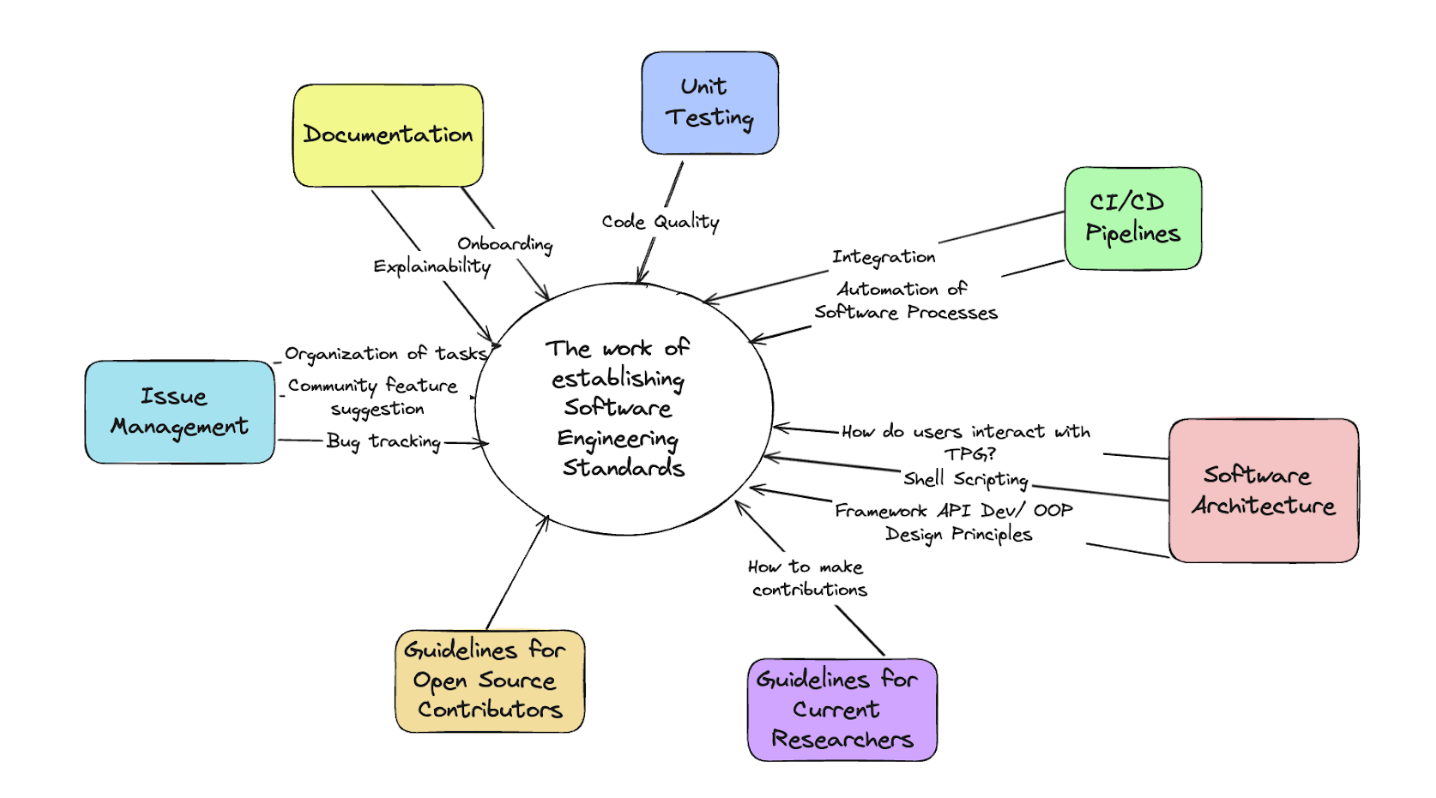
\includegraphics[scale=0.6]{SystemContext.png}
  \caption{System Context}
  \label{Fig_SystemContext} 
  \end{center}
\end{figure}

\begin{itemize}
  \item Unit Testing: Focused on improving code quality, unit tests ensure that individual pieces of the codebase work as expected.
  \item CI/CD Pipelines: The integration and automation of software processes, such as building and testing, will allow for continuous integration and deployment of changes, ensuring the project remains robust as it scales.
  \item Software Architecture: This examines how users interact with TPG, the use of shell scripting, and how the framework is structured using API development and object-oriented programming (OOP) principles. It emphasizes improving design principles for a better developer and user experience.
  \item Documentation: This is critical for onboarding new developers, ensuring explainability, and providing clear, thorough project documentation.
  \item Issue Management: Introducing a formal system to track bugs, feature requests, and community suggestions will help organize tasks and streamline project development.
  \item Guidelines for Open Source Contributors: Establishing clear guidelines will provide a roadmap for external contributors to participate in the project, increasing collaboration and contributions.
  \item Guidelines for Current Researchers: This component covers how researchers and developers within the project can contribute effectively, ensuring consistency and alignment with the project's goals.
\end{itemize}

\subsubsection{Physics Engine Integration}
\begin{figure}[hbt!]
  \begin{center}
   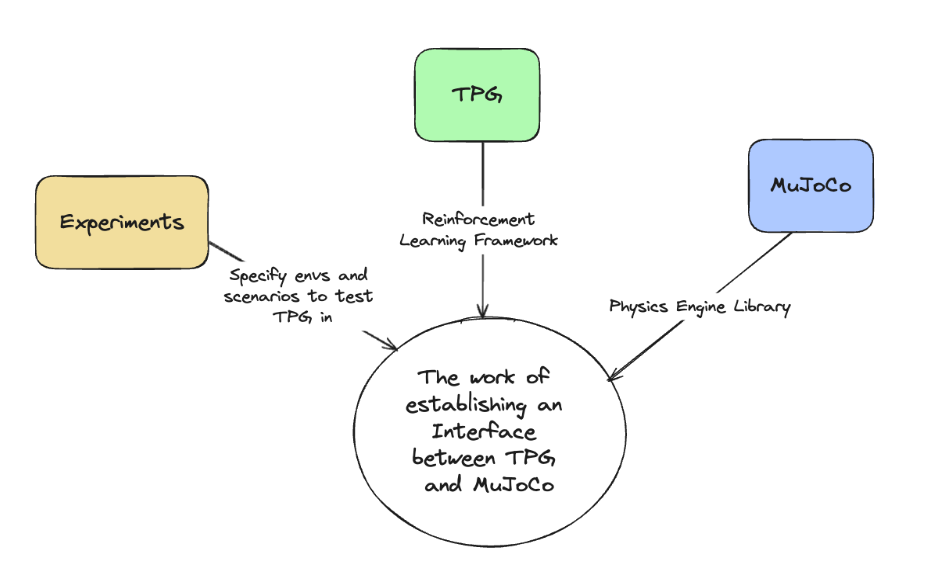
\includegraphics[scale=0.5]{PhysicsEngineContext.png}
  \caption{System Context}
  \label{Fig_PhysicsEngineContext} 
  \end{center}
\end{figure}

\begin{itemize}
  \item TPG (Tangled Program Graphs): TPG is a reinforcement learning framework. In this context, its role is to act as the core system that will be tested and integrated with dynamic environments. Establishing the interface between TPG and MuJoCo will allow the TPG framework to be tested in physically realistic simulations.
  \item MuJoCo (Multi-Joint dynamics with Contact): MuJoCo is a high-performance physics engine used for modeling and simulating dynamic systems. In this diagram, it represents the external library that provides the physics-based environments required for testing TPG. The interface with TPG will enable the reinforcement learning agents created using TPG to interact with complex, real-world-like physics simulations provided by MuJoCo.
  \item Experiments: Experiments define the environments and scenarios where TPG will be tested. This component represents the experimental setups that specify the parameters for evaluating TPG’s performance in various MuJoCo-based scenarios. These experiments are critical for determining how well TPG adapts to different physics-based tasks, environments, and scenarios.
\end{itemize}

\subsection{Work Partitioning}

\begin{xltabular}{\textwidth}{   
  | >{\raggedright\arraybackslash}X 
  | >{\raggedright\arraybackslash}X 
  | >{\raggedright\arraybackslash}X 
  | >{\raggedright\arraybackslash}X | }
  \caption{Work Partitioning Table} \\
  
  \hline \multicolumn{1}{|c|}{\textbf{Event Name}} & \multicolumn{1}{c|}{\textbf{Inputs}} & \multicolumn{1}{c|}{\textbf{Outputs}} & \multicolumn{1}{c|}{\textbf{Summary}} \\ \hline 
  \endfirsthead
  
  \multicolumn{4}{c}%
  {\tablename\ \thetable{} -- continued from previous page} \\
  \hline \multicolumn{1}{|c|}{\textbf{Event Name}} & \multicolumn{1}{c|}{\textbf{Inputs}} & \multicolumn{1}{c|}{\textbf{Outputs}} & \multicolumn{1}{c|}{\textbf{Summary}} \\ \hline 
  \endhead
  
  \hline \multicolumn{4}{|r|}{{Continued on next page}} \\ \hline
  \endfoot
  \hline
\endlastfoot
\hline
Contributor wants to merge code changes they made & New changes (code that was modified in a PR) & New code is successfully integrated with the main code & CI - Continuous Integration practices into the repo, ensuring all devs can make changes in a seamless manner and be up to date while concurrent work is occuring \\
\hline
Contributor wants to evaluate the code they wrote & New code blocks that are written by a contributor & Test functions are created to evaluate new code & Automated tests are generated for new code blocks that are written ensuring code robustness \\
\hline
Contributor wants to onboard and use TPG & N/A & Contributor is able to run the framework & Seamless onboarding experience that allows a new contributor/user to get up and running \\
\hline
Contributor wants to perform an experiment to test the TPG framework in MuJoCo & TPG, MuJoCo & Functioning simulation of an experiment integrated with a physics engine & New experiments to be conducted in more realistic scenarios evolving the development of this reinforcement learning framework \\
\hline
Contributor wants to get visual results of from test data & TPG, MuJoCo & Graphs of the recent experiment & Evaluation of the experiment is crucial to improving the framework and allowing it to become good at multi task reinforcement learning tasks \\

\end{xltabular}

\section{Business Data Model and Data Dictionary}
\subsection{Business Data Model}
\subsubsection{Software Engineering Practices}

\begin{figure}[ht!]
  \begin{center}
   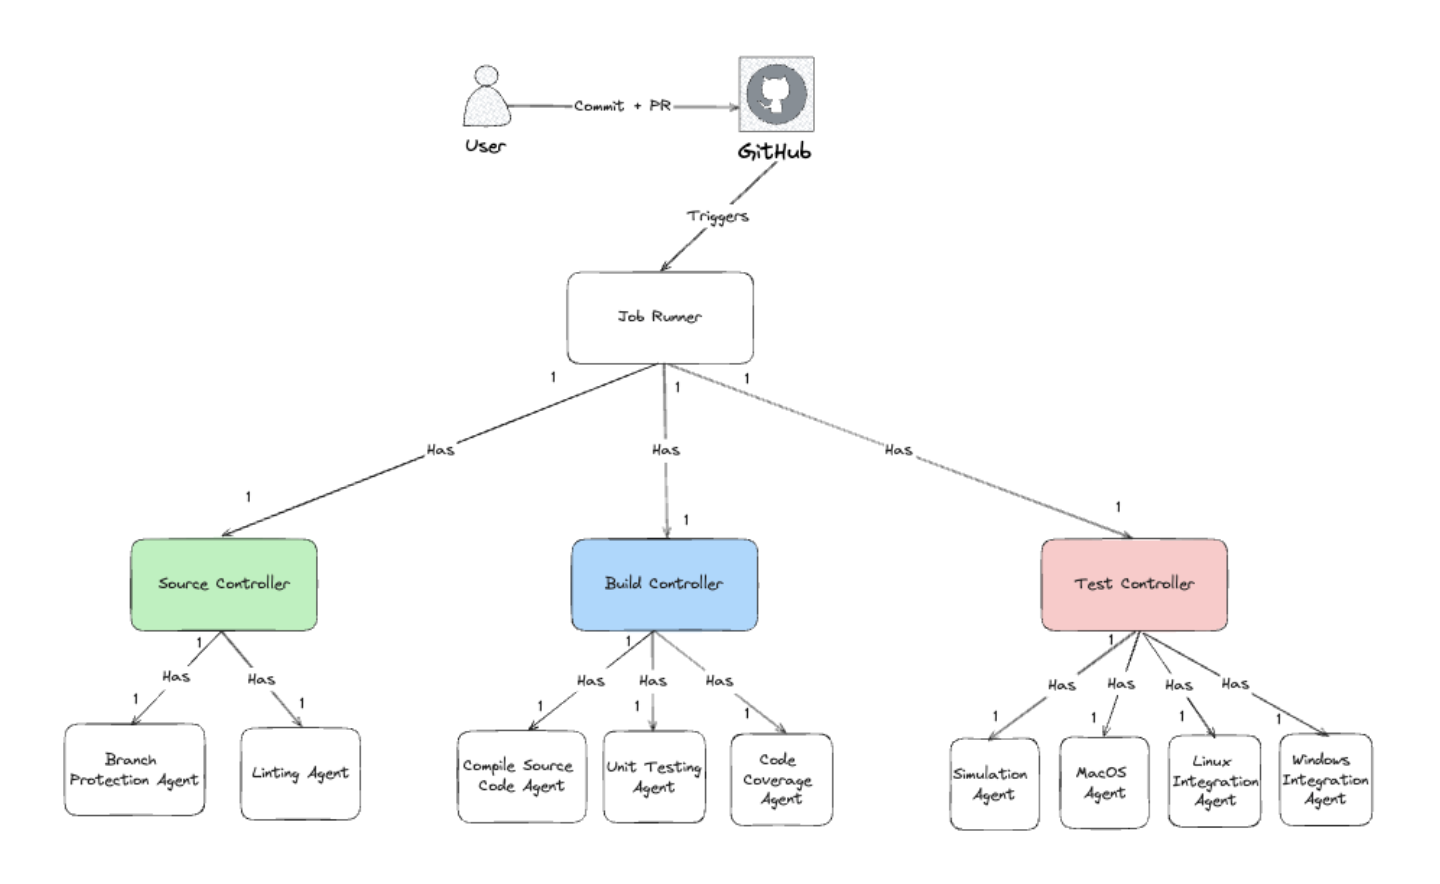
\includegraphics[scale=0.5]{DataModel.png}
  \caption{Data Model}
  \label{Fig_DataModel} 
  \end{center}
\end{figure}

\clearpage

Figure 3 illustrates a UML data model of a traditional CI/CD pipeline implemented using GitHub Actions. The architecture follows a master-slave design pattern, where the pipeline steps are defined in a YAML configuration file. For each step in the pipeline, a Controller (master) class orchestrates the process by delegating tasks to Agents (slaves) that handle specific actions. This design is commonly used in CI/CD pipelines because it reflects the sequential nature of the CI/CD process—each step must wait for the previous one to complete before proceeding.

\subsubsection{Physics Engine Integration}

\begin{figure}[ht!]
  \begin{center}
   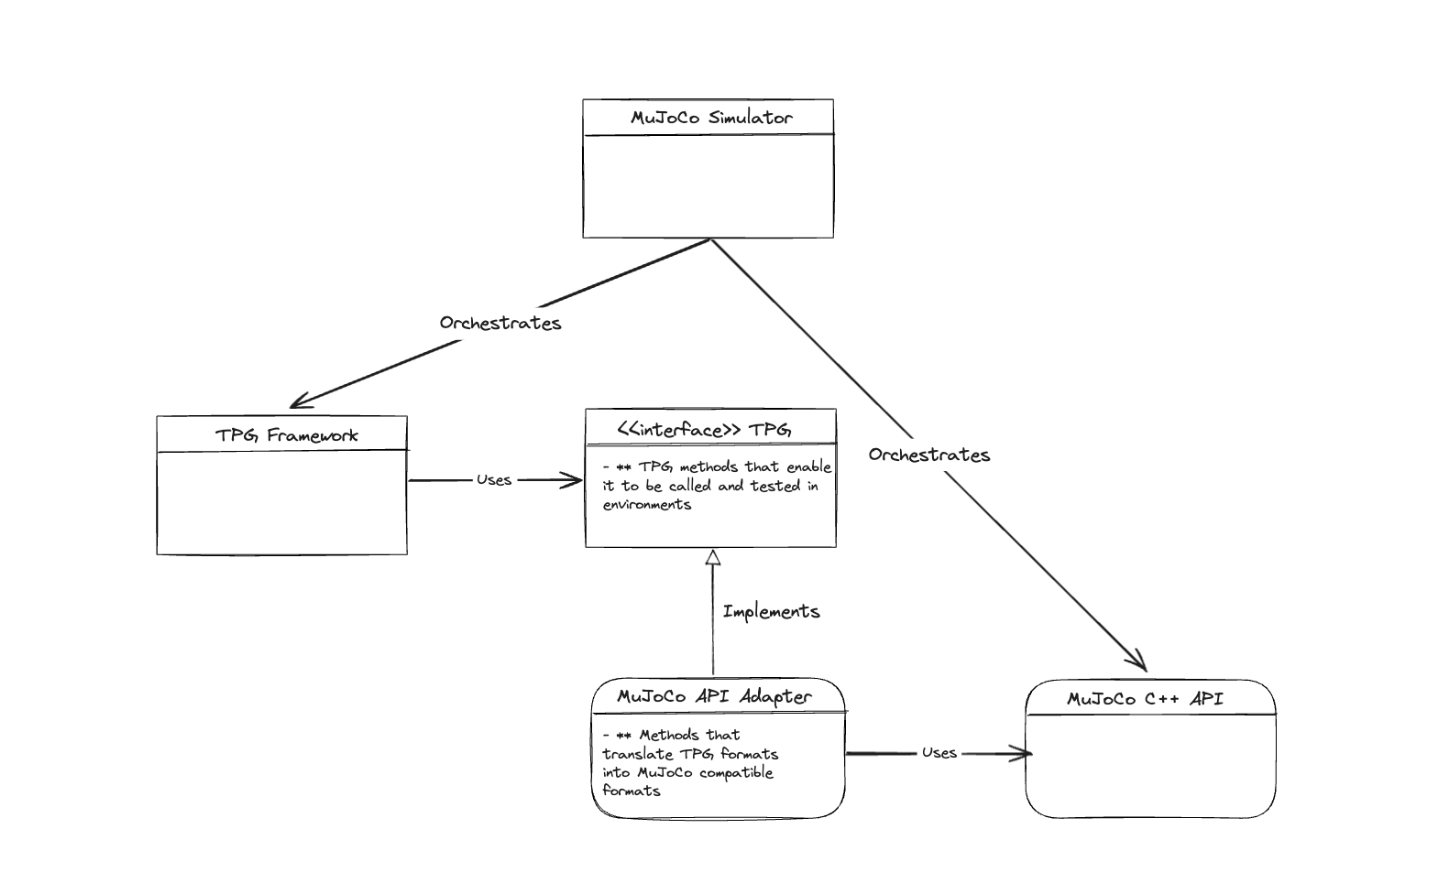
\includegraphics[scale=0.5]{ClassModel.png}
  \caption{Physics Engine Class Diagram}
  \label{Fig_ClassModel} 
  \end{center}
\end{figure}

Figure 4 presents a simplified UML data model of the interface being developed to integrate the TPG framework with MuJoCo. The primary objective is to adapt how the TPG framework handles state changes into a format that MuJoCo can interpret. To achieve this, we are utilizing the Adapter design pattern to translate incompatible formats and ensure compatibility between the two systems.

\subsection{Data Dictionary}

\begin{xltabular}{\textwidth}{   
  | >{\raggedright\arraybackslash}X 
  | >{\raggedright\arraybackslash}X 
  | >{\raggedright\arraybackslash}X | }
  \caption{Data Dictionary Table} \\
  
  \hline \multicolumn{1}{|c|}{\textbf{Name}} & \multicolumn{1}{c|}{\textbf{Content}} & \multicolumn{1}{c|}{\textbf{Type}} \\ \hline 
  \endfirsthead
  
  \multicolumn{3}{c}%
  {\tablename\ \thetable{} -- continued from previous page} \\
  \hline \multicolumn{1}{|c|}{\textbf{Name}} & \multicolumn{1}{c|}{\textbf{Content}} & \multicolumn{1}{c|}{\textbf{Type}} \\ \hline 
  \endhead
  
  \hline \multicolumn{3}{|r|}{{Continued on next page}} \\ \hline
  \endfoot
  \hline
\endlastfoot
\hline
Job Runner & Orchestrates all the jobs for the GitHub Actions CI/CD Pipeline & Class \\
\hline
Source Controller & Responsible for orchestrating Branch Protection rules and Linting during the Source stage of the CI/CD Pipeline & Class \\
\hline
Branch Protection Agent & Responsible for enabling branch protection on the repo to prevent accidental integrations on the main branch & Class \\
\hline
Linting Agent & Static analysis on the code and cleans it up & Class \\
\hline
Build Controller & Responsible for orchestrating the Build stage of the CI/CD Pipeline & Class \\
\hline
Compile Source Code Agent & Compiles the code to prepare it for validation & Class \\
\hline
Unit Testing Agent & Runs through all the unit tests in an automated fashion & Class \\
\hline
Code Coverage Agent & Static analyzes the coverage from the unit tests, usually needs to be above 85\% & Class \\
\hline
Test Controller & Responsible for orchestrating the Test stage of the CI/CD Pipeline & Class \\
\hline
MacOS, Linux, Windows Agents & Containers for each OS to test the integration of the framework in each environment (industry standard) & Class \\
\hline
Simulation Agent & Responsible for integration testing to ensure the new changes are robust and don’t break & Class \\

\end{xltabular}

\section{The Scope of the Product}
\subsection{Product Boundary}

\begin{xltabular}{\textwidth}{   
  | >{\raggedright\arraybackslash}X 
  | >{\raggedright\arraybackslash}X | }
  \caption{Product Boundary} \\
  
  \hline \multicolumn{1}{|c|}{\textbf{In Scope}} & \multicolumn{1}{c|}{\textbf{Out of Scope}} \\ \hline 
  \endfirsthead
  
  \multicolumn{2}{c}%
  {\tablename\ \thetable{} -- continued from previous page} \\
  \hline \multicolumn{1}{|c|}{\textbf{In Scope}} & \multicolumn{1}{c|}{\textbf{Out of Scope}} \\ \hline 
  \endhead
  
  \hline \multicolumn{2}{|r|}{{Continued on next page}} \\ \hline
  \endfoot
  \hline
\endlastfoot
\hline
CI/CD Pipeline: Software Engineering practices need to be integrated into the code base & Ongoing research experiments with TPG: Since Dr. Kelly and his grad students are still developing TPG, the scope of our capstone won’t encompass current efforts \\
\hline
Interface between MuJoCo + TPG: Development of the interface that enables testing and evaluation of TPG in a physics engine must be established & \\
\hline
Code refactoring: Reorganizing code structure to make it suitable as a C API to allow open source contributions/seamless integrations into other projects & \\

\end{xltabular}

\subsection{Product Use Case Table}

\begin{xltabular}{\textwidth}{   
  | >{\raggedright\arraybackslash}X 
  | >{\raggedright\arraybackslash}X | }
  \caption{Product Boundary} \\
  
  \hline \multicolumn{1}{|c|}{\textbf{User}} & \multicolumn{1}{c|}{\textbf{Use Case}} \\ \hline 
  \endfirsthead
  
  \multicolumn{2}{c}%
  {\tablename\ \thetable{} -- continued from previous page} \\
  \hline \multicolumn{1}{|c|}{\textbf{User}} & \multicolumn{1}{c|}{\textbf{Use Case}} \\ \hline 
  \endhead
  
  \hline \multicolumn{2}{|r|}{{Continued on next page}} \\ \hline
  \endfoot
  \hline
\endlastfoot
\hline

\multirow{2}{0.5\textwidth}{Researchers in Dr. Kelly’s research group} & - When researcher make changes to the code base, they are able to validate their logic through unit testing, integration testing in the CI/CD pipeline \\
& - Perform experimentations using TPG in a physics engine, to further improve the reinforcement learning framework \\
& - Access the code not by only using shell scripts, but through the C API \\
& - Share how the integration is done in an Open Source manner to allow other community members to access the code \\
& - Issue management to organize who is working on what currently \\

\multirow{2}{0.5\textwidth}{Open Source Contributors} & - Access and embed the TPG framework into their own applications \\
& - Make changes to the TPG framework in an automated manner \\
& - Suggest changes to the framework in an standardized way \\

\end{xltabular}

\subsection{System Boundaries}
\subsubsection{GitHub Actions Pipeline}

\begin{figure}[ht!]
  \begin{center}
   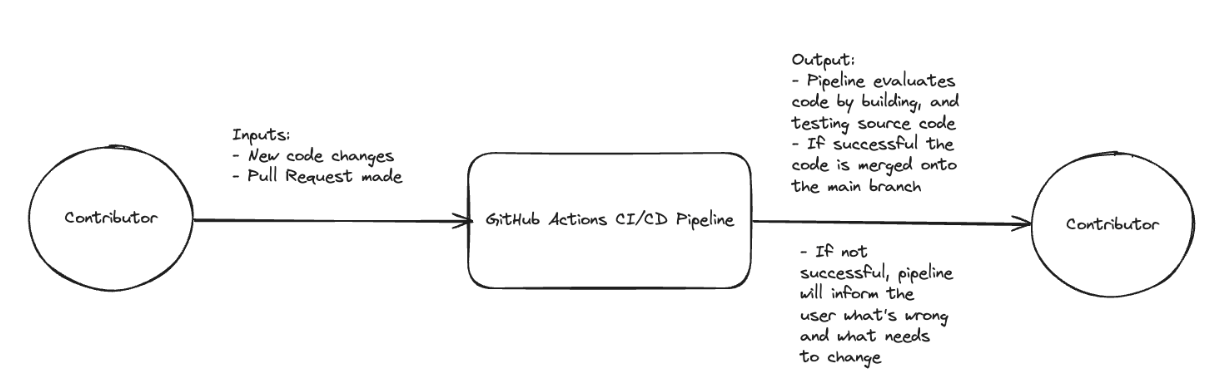
\includegraphics[scale=0.5]{GitHubActionsSystem.png}
  \caption{GitHub Actions Pipeline System Boundary}
  \label{Fig_GitHubActions} 
  \end{center}
\end{figure}

\subsubsection{Physics Engine Integration}

\begin{figure}[ht!]
  \begin{center}
   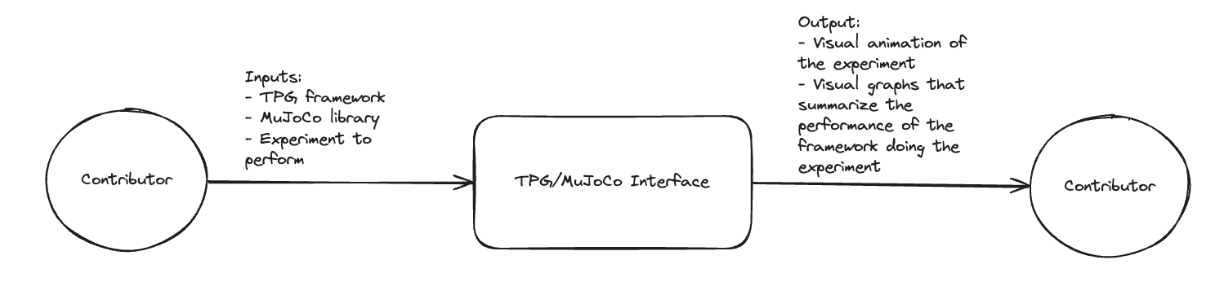
\includegraphics[scale=0.5]{PhysicsIntegration.png}
  \caption{MuJoCo Physics Integration}
  \label{Fig_MuJoCo} 
  \end{center}
\end{figure}

\subsection{Formalized Math and Application Flow}
\subsubsection{Software Engineering Practices}

Definitions: Let C be the set of all code changes, T be the set of all tests, S be the set of all test successes, E be the set of all test failures

Functions:
\begin{enumerate}
  \item \begin{math}
    Success: C \cap T \rightarrow S
  \end{math}
  \item \begin{math}
    Failure: C \cap T \rightarrow E
  \end{math}
\end{enumerate}

\subsubsection{Physics Engine Integration}

Definitions: Let T represent the TPG framework, M represent the MuJoCo framework, E represent the experiment

Relation:
\begin{enumerate}
  \item \begin{math}
    R \subseteq E \cup (T \cap M)
  \end{math}
\end{enumerate}

\section{Functional Requirements}
\subsection{Functional Requirements}
\lips

\section{Look and Feel Requirements}
\subsection{Appearance Requirements}
\lips
\subsection{Style Requirements}
\lips

\section{Usability and Humanity Requirements}
\subsection{Ease of Use Requirements}
\lips
\subsection{Personalization and Internationalization Requirements}
\lips
\subsection{Learning Requirements}
\lips
\subsection{Understandability and Politeness Requirements}
\lips
\subsection{Accessibility Requirements}
\lips

\section{Performance Requirements}
\subsection{Speed and Latency Requirements}
\lips
\subsection{Safety-Critical Requirements}
\lips
\subsection{Precision or Accuracy Requirements}
\lips
\subsection{Robustness or Fault-Tolerance Requirements}
\lips
\subsection{Capacity Requirements}
\lips
\subsection{Scalability or Extensibility Requirements}
\lips
\subsection{Longevity Requirements}
\lips

\section{Operational and Environmental Requirements}
\subsection{Expected Physical Environment}
\lips
\subsection{Wider Environment Requirements}
\lips
\subsection{Requirements for Interfacing with Adjacent Systems}
\lips
\subsection{Productization Requirements}
\lips
\subsection{Release Requirements}
\lips

\section{Maintainability and Support Requirements}
\subsection{Maintenance Requirements}
\lips
\subsection{Supportability Requirements}
\lips
\subsection{Adaptability Requirements}
\lips

\section{Security Requirements}
\subsection{Access Requirements}
\lips
\subsection{Integrity Requirements}
\lips
\subsection{Privacy Requirements}
\lips
\subsection{Audit Requirements}
\lips
\subsection{Immunity Requirements}
\lips

\section{Cultural Requirements}
\subsection{Cultural Requirements}
\lips

\section{Compliance Requirements}
\subsection{Legal Requirements}
\lips
\subsection{Standards Compliance Requirements}
\lips

\section{Open Issues}
\lips

\section{Off-the-Shelf Solutions}
\subsection{Ready-Made Products}
\lips
\subsection{Reusable Components}
\lips
\subsection{Products That Can Be Copied}
\lips

\section{New Problems}
\subsection{Effects on the Current Environment}
\lips
\subsection{Effects on the Installed Systems}
\lips
\subsection{Potential User Problems}
\lips
\subsection{Limitations in the Anticipated Implementation Environment That May
Inhibit the New Product}
\lips
\subsection{Follow-Up Problems}
\lips

\section{Tasks}
\subsection{Project Planning}
\lips
\subsection{Planning of the Development Phases}
\lips

\section{Migration to the New Product}
\subsection{Requirements for Migration to the New Product}
\lips
\subsection{Data That Has to be Modified or Translated for the New System}
\lips

\section{Costs}
\lips
\section{User Documentation and Training}
\subsection{User Documentation Requirements}
\lips
\subsection{Training Requirements}
\lips

\section{Waiting Room}
\lips

\section{Ideas for Solution}
\lips

\newpage{}
\section*{Appendix --- Reflection}

The information in this section will be used to evaluate the team members on the
graduate attribute of Lifelong Learning.  Please answer the following questions:

\begin{enumerate}
  \item What knowledge and skills will the team collectively need to acquire to
  successfully complete this capstone project?  Examples of possible knowledge
  to acquire include domain specific knowledge from the domain of your
  application, or software engineering knowledge, mechatronics knowledge or
  computer science knowledge.  Skills may be related to technology, or writing,
  or presentation, or team management, etc.  You should look to identify at
  least one item for each team member.
  \item For each of the knowledge areas and skills identified in the previous
  question, what are at least two approaches to acquiring the knowledge or
  mastering the skill?  Of the identified approaches, which will each team
  member pursue, and why did they make this choice?
\end{enumerate}

\end{document}